%Bibliometria. Cientometria. Impacto de pesquisa.

\section{Comentários iniciais}

%%
\begin{frame}{Comentários}
\begin{itemize}
\item ``Bibliometria'', ``cientometria'' e ``infometria'' destinam-se à mensuração da ciência
\item Disciplinas da Ciência da Informação que estudam a dinâmica da produção de literatura
\item A ciência que estuda a própria ciência
\item Crescimento, estrutura, inter-relacionamento e produtividade
\item Mais recentemente, cunhou-se o termo ``webmetria''\footnote{Parece não haver consenso na tradução desses termos. Usam-se também: ``cienciometria'', ``informetria'', ``webometria'', ``cibermetria'', ``internetometria''.}
\end{itemize}
\end{frame}

%%
\begin{frame}{Utilidade}
Avaliar a produção científica é útil para
\begin{itemize}
\item estabelecer políticas nacionais de ensino e pesquisa
\item diagnosticar e monitorar potencialidades e fraquezas de grupos e instituições
\item mensurar a produtividade de pesquisadores
\item medir a difusão do conhecimento científico e o fluxo da informação
\item fatores de impacto com base em densidade de \emph{links}.
\end{itemize}
\end{frame}

%%
\begin{frame}{Relação com mapeamento sistemático}
\begin{itemize}
\item Bibliometria em termos de quantificação se relaciona com MS 
\item Mapeamento da pesquisa em um campo em ampla escala 
\item Documentação do tamanho, trajetória de crescimento e distribuição geográfica de um tópico
\end{itemize}
\end{frame}

%%
\begin{frame}{Exemplo}

O material seguinte foi extraído do artigo: \textit{A Bibliometric Review of Research on Educational Administration: Science Mapping the Literature, 1960 to 2018}, de autoria de P. Hallinger e J. Kovacevic. doi: 10.3102/0034654319830380.

\end{frame}

\begin{frame}{Busca e filtragem de fontes}
Método aplicado pelos autores
\begin{figure}
\centering
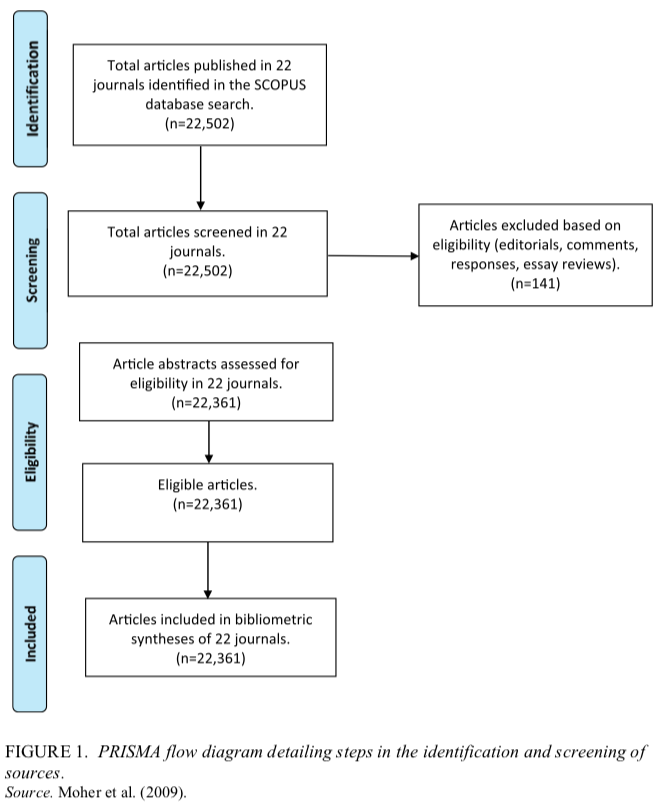
\includegraphics[scale=0.25]{figs/03/exemplo-1-1}
\end{figure}
\end{frame}

\begin{frame}{Links}
\begin{figure}
\centering
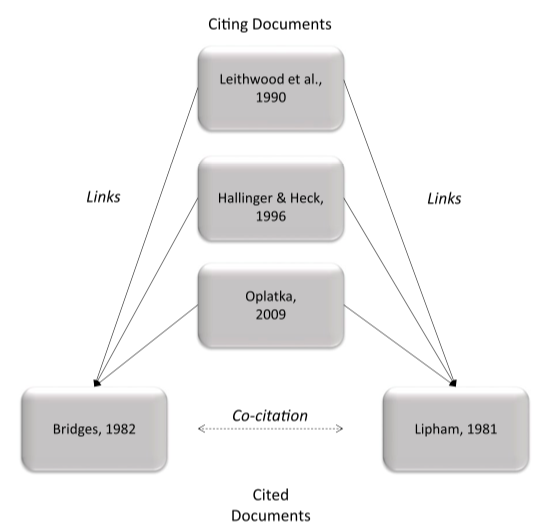
\includegraphics[scale=0.35]{figs/03/exemplo-1-2}
\end{figure}
\end{frame}

\begin{frame}{Mapa geográfico}
\begin{figure}
\centering
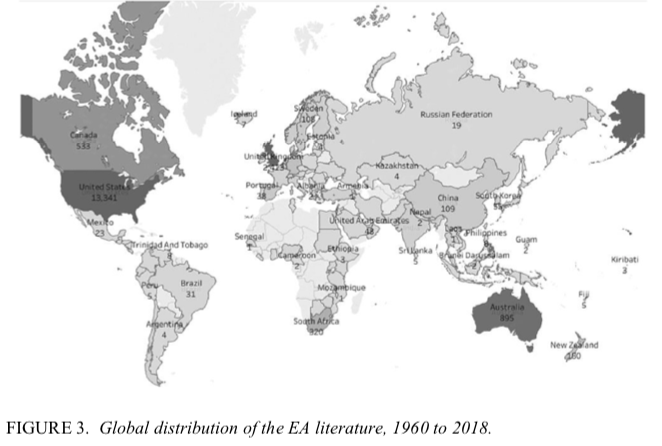
\includegraphics[scale=0.45]{figs/03/exemplo-1-3}
\end{figure}
\end{frame}

\begin{frame}{Rede de citações/co-citações}
\begin{figure}
\centering
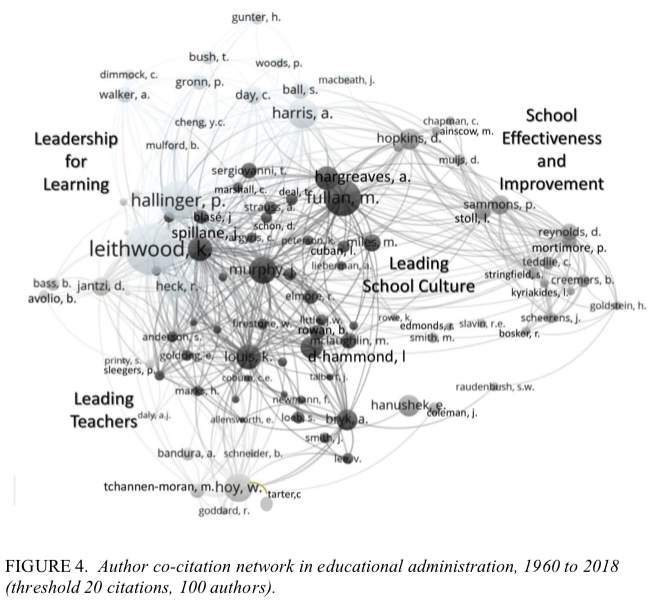
\includegraphics[scale=0.35]{figs/03/exemplo-1-4}
\end{figure}
\end{frame}

\begin{frame}{Mapa de co-ocorrências}
\begin{figure}
\centering
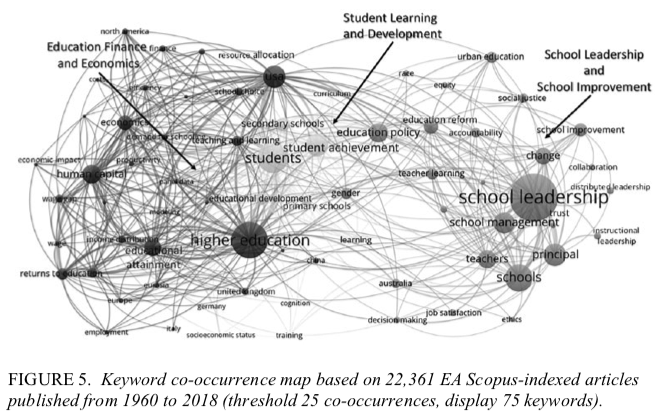
\includegraphics[scale=0.45]{figs/03/exemplo-1-5}
\end{figure}
\end{frame}

\section{Métricas da literatura}

%%
\begin{frame}{Bibliometria}
\begin{itemize}
\item Índices de citação (1743); contagens de publicação (1817)\footnote{Segundo historiadores da Ciência da Informação}
\item Primeiro estudo bibliométrico: Campbell (1896)
\item Primeiros trabalhos: Cole \& Eales (1917), Hulme (1923)
\end{itemize}
\begin{block}{Bibliometria}
``A aplicação de métodos matemáticos e estatísticos a livros e outros meios de comunicação.''
(Pritchard, 1969).
\end{block}
\end{frame}

%%
\begin{frame}{Cientometria}
\begin{itemize}
\item Surge em 1969 com o russo Vassily Nalimov
\item Expande-se em 1978 quando Tibor Braun funda o periódico \textit{Scientometrics}\footnote{Gerido pela Springer:
 \url{https://link.springer.com/journal/11192}.}
\item Inclui aspectos quantitativos da ciência da ciência, comunicação e política da ciência
\item Não possui definição clara, mas concentra-se em estudar (Hood, 2001, \emph{apud:} Wilson, 2001): 
\begin{itemize}
\item práticas de pesquisadores;
\item gestão de pesquisa e desenvolvimento
\item o papel da C{\&}T na economia e na política nacional 
\end{itemize}
\end{itemize}
\end{frame}

%%
\begin{frame}{Infometria} 
\begin{itemize}
\item Proposto primeiramente por Nacke em 1979
\item Termo criado com o objetivo de medir fenômenos da informação
\item Usa métodos matemáticos para recuperação da informação (\textit{information retrieval})
\end{itemize}
\end{frame}

%%
\begin{frame}{Webmetria}
\begin{itemize}
\item Aplica métodos da infometria à rede mundial de computadores (web)
\item Atribui-se a autoria do termo a Almind e Ingwersen (1997)
\item Web como canal de comunicação científica 
\item Estudos quantitativos neste ambiente
\end{itemize}
\end{frame}

%%
\begin{frame}{Quadro comparativo}
\begin{figure}
\centering
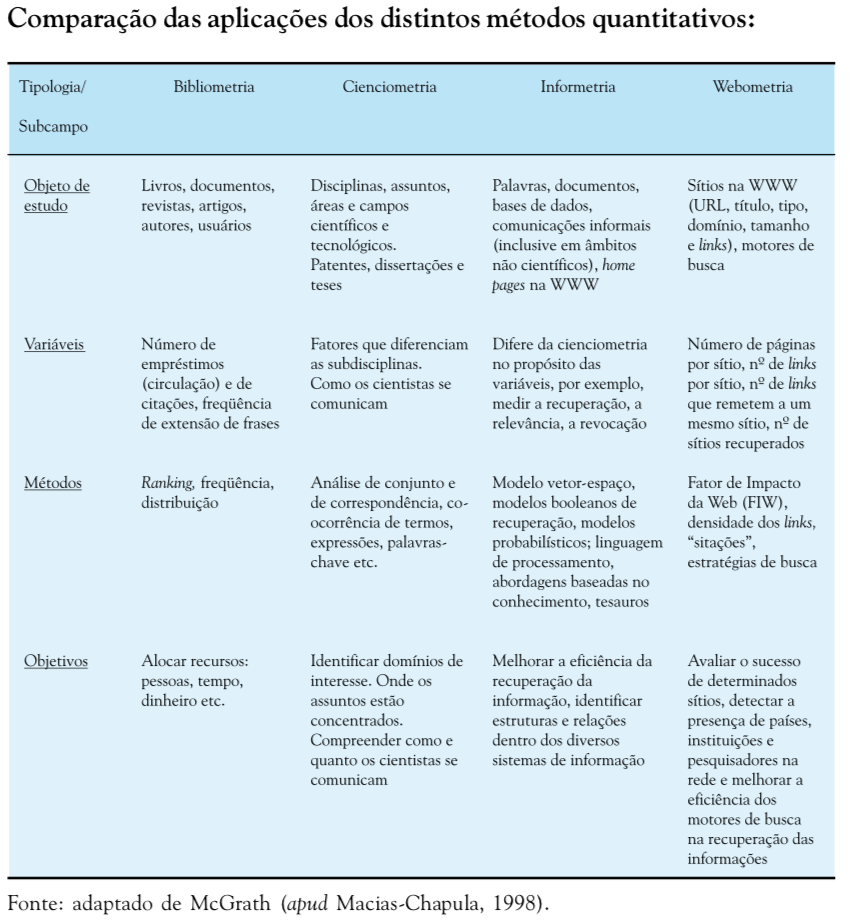
\includegraphics[scale=0.2]{figs/03/quadro-metricas}
\caption{Fonte: Vanti (2002).}
\end{figure}
\end{frame}

\begin{frame}{Diagrama}
\begin{figure}
\centering
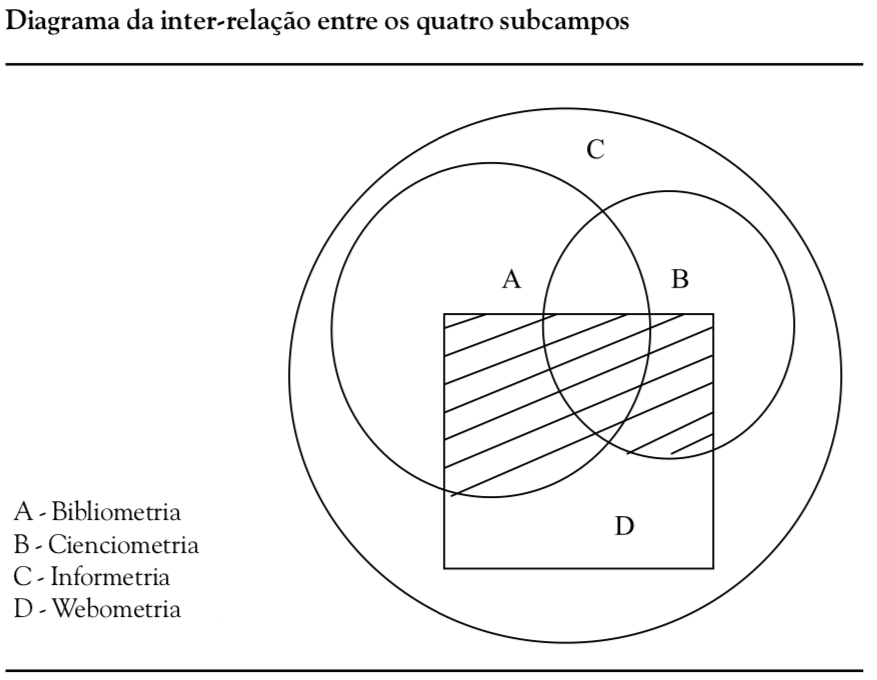
\includegraphics[scale=0.2]{figs/03/diagrama-metricas}
\caption{Fonte: Vanti (2002).}
\end{figure}
\end{frame}

%%
\begin{frame}{Aplicações de técnicas das x-metrias}
\begin{itemize}
\item identificação de tendências e crescimento do conhecimento em uma área
\item detecção de revistas do núcleo de uma disciplina, bem como as secundárias 
\item previsão das tendências de publicação
\item análise de citações e co-citações 
\item entre outras... 
\end{itemize}
Ver: \texttt{http://www.scielo.br/pdf/ci/v31n2/12918}
\end{frame}

\section{Fatores de impacto}

%%
\begin{frame}{Entendendo a jornada...}
\begin{itemize}
\item Projeto pioneiro de Eugene Garfield: \emph{Institute for Scientific Information} - ISI (década de 1960) 
\item ISI oferecia serviços bibliográficos e cientométricos 
\item Especialidade do ISI era o seu \emph{Science Citation Index} - SCI
\item O ISI também abrangia o \emph{Social Sciences Citation Index} - SSCI e o \emph{Arts and Humanities Citation Index} - AHCI
\end{itemize}
\end{frame}

%%
\begin{frame}{cont.}
\begin{itemize}
\item Em 1992, o ISI foi adquirido pela multinacional Thomson Reuters 
\item Aqui surge a antiga Web of Knowledge
\item Em 2016, a TR vende sua parte no negócio para outras empresas que formam a Clarivate Analytics
\item Até hoje a Clarivate Analytics é proprietária da conhecida \textbf{Web of Science - WoS}
\item A partir de 2000 em diante, competidores aparecem: Elsevier Scopus e Google Scholar (2004)
\end{itemize}
\end{frame}

%% 
\begin{frame}{A produção científica é um nicho de mercado}
\begin{figure}
\centering

\includegraphics[scale=0.4]{figs/03/the-scientist}
\caption{Matéria publicada no \textit{The Scientist} em 15/07/2016. Disponível em: 
\url{https://www.the-scientist.com/the-nutshell/web-of-science-sold-for-more-than-3-billion-33184}.}
\end{figure}
\end{frame}

%%
\begin{frame}{Definições básicas}
\begin{block}{Citação}
Uma referência a uma fonte publicada ou não publicada. 
\end{block}
\begin{block}{Índice de citação}
Tipo de Índice bibliográfico utilizado na pesquisa científica para organizar citações entre publicações
\end{block}
\begin{block}{Serviços de indexação de citações\footnote{Predominantes: 
Web of Science, Scopus, CiteSeer, Google Scholar, PubMed}}
Um banco de dados que fornece ao usuário um aparato organizado para localização rápida de publicações e referências
\end{block}
\end{frame}

\begin{frame}{cont.}
\begin{block}{Métrica de citação\footnote{Relaciona-se à bibliometria, cientometria.}}
Quantificador do impacto de citações de trabalhos acadêmicos.
\end{block}
\begin{block}{Fator de impacto}
Índice cientométrico que reflete a importância relativa de um periódico.
\end{block}
\begin{block}{Periódico (\emph{Journal})}
Publicação periódica onde a pesquisa científica é apresentada e discutida. São coloquialmente chamados de ``revista''.
(Atenção! Jornal = \emph{newspaper})
\end{block}
\end{frame}

\begin{frame}{Níveis de impacto}
O impacto da produção científica é medido em dois níveis por métricas matematicamente definidas
\begin{itemize}
\item \textbf{Quanto ao periódico}: estimado pelo \textit{fator de impacto do periódico} (\textit{Journal Impact Factor})
\item \textbf{Quanto ao artigo}: estimado por métricas alternativas que consideram a interação social
\item \textbf{Quanto ao autor}: estimado por um \textit{índice de citação}
\end{itemize}
\end{frame}

\subsection*{Métricas de períodicos}

%%
\begin{frame}{\textit{Journal Impact Factor}}
Número médio de citações dos artigos publicados pelo periódico durante uma janela temporal(em geral, 1 a 5 anos).

\begin{block}{Cálculo do JIF para um dado ano $t$}
\[
JIF(t) = \dfrac{C(t-1) + C(t-2)}{P(t-1) + P(t-2)}
\]
\begin{itemize}
\item $C$: número de citações 
\item $P$: número de publicações
\end{itemize}
\end{block}
\end{frame}

%%
\begin{frame}{Outras medidas}
\begin{itemize}
\item Autofator \textit{(Eigenfactor)}
\item SCImago Journal Rank: ver \url{https://www.scimagojr.com} 
\item PageRank
\item JRank
\end{itemize}
\end{frame}

%%
\begin{frame}{\textit{Journal Citation Report}}

Uma ferramenta online que ranqueia o valor e impacto de um periódico com base em métricas e análise de dados.  Disponível \url{https://clarivate.com/products/journal-citation-reports/}. Acessível com login institucional (veremos adiante). 

Como o JCR 2019 calculou o JIF? 

Veja: \url{https://clarivate.com/webinars/journal-citation-reports-2019-update/}
\end{frame}

\subsection*{Métricas de artigos}

\begin{frame}{Métricas de artigos}
\begin{quotation}
\textit{``Article-Level Metrics (ALMs) seek to incorporate new data sources along with traditional measures to present a richer picture of how an individual article is being discussed, shared, and used.''} (SPARC)
\end{quotation}
\begin{itemize}
\item Uso: quantas vezes o artigo foi visualizado? 
\item Capturas: quantas um artigo foi marcado e compartilhado?
\item Menções: com que frequencia falam sobre o artigo?
\item Mídias sociais: quantos likes no FB, Linkedin ou outras redes? 
\end{itemize}

Ver: \url{https://sparcopen.org/our-work/article-level-metrics/}
\end{frame}

%%
\begin{frame}{ALM: longevidade x imediatismo; granularidade x agregação}
\begin{figure}
\centering
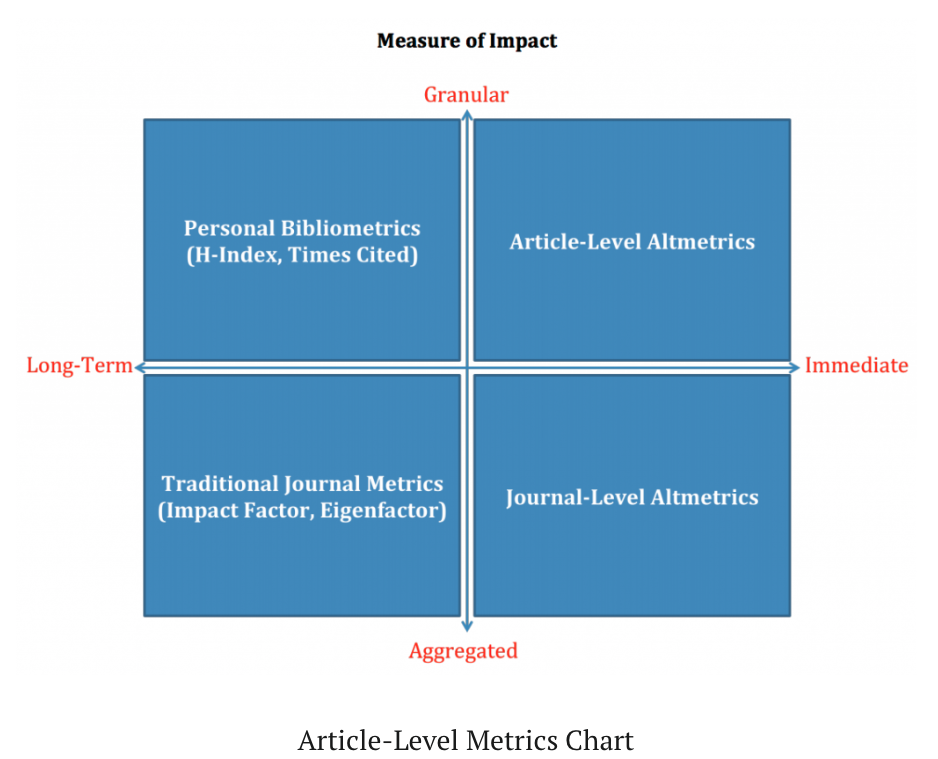
\includegraphics[scale=0.2]{figs/03/alm}
\caption{Medida de impacto. Fonte: SPARC}
\end{figure}
\end{frame}

\subsection*{Métricas de autor}

%%
\begin{frame}{Métricas do cientista}
\begin{itemize}
\item Medem o impacto das citações das publicações de um cientista
\item Meio de refletir importância e produtividade
\item A métrica mais conhecida e utilizada é o \textit{índice h} (de Hirsch), proposto por J. E. Hirsch (2005)
\item Existem outros índices, mas menos conhecidos: $m$, $g$, $s$ e $c$. 
\item Há diversas críticas sobre o índice $h$
\end{itemize}
\end{frame}

%%
\begin{frame}{\textit{Highly Cited Researchers}}

\begin{quotation}
\textit{``A list of elite scientists and social scientists identified through analysis of highly cited papers (those ranking in the top 1\% by citations for field and year).''}
\end{quotation}

Ver: \url{https://hcr.clarivate.com}.

\end{frame}


%%
\begin{frame}{O índice $h$}
\begin{quotation}
``Um cientista tem índice $h$ se $h$ de seus $N$ artigos publicados têm pelo menos $h$ citações cada, e os outros $(N-h)$ artigos não tiverem mais do que $h$ citações.'' (Hirsch, 2005).
\end{quotation}

Ver: \url{https://www.ncbi.nlm.nih.gov/pmc/articles/PMC1283832/pdf/pnas-0507655102.pdf}
\end{frame}

%%
\begin{frame}{Entendendo o índice $h$...}
\begin{figure}
\centering
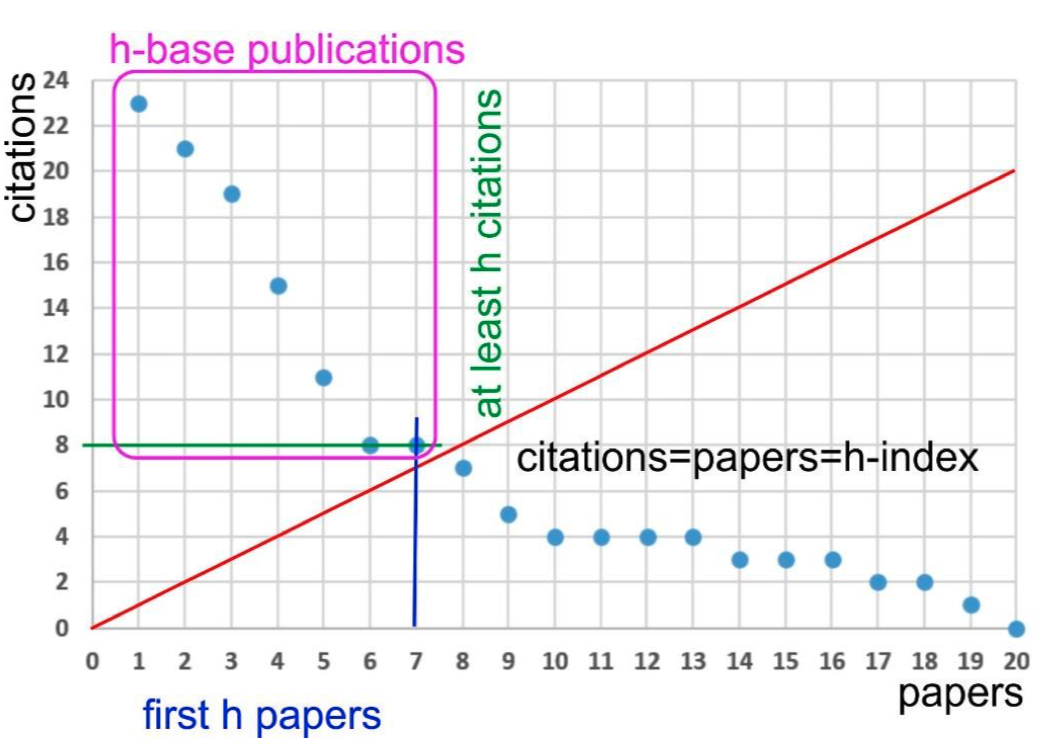
\includegraphics[scale=0.2]{figs/03/h-index}
\caption{Índice $h$. Fonte: Wikipedia.}
\end{figure}
\end{frame}

%%
\begin{frame}{Críticas ao índice $h$}
Algumas são:
\begin{itemize}
\item Desconsidera o número de citações em campos do conhecimento diferentes
\item É um número natural
\item Pode ser manipulado através de autocitações
\end{itemize}
\end{frame}

%%
\begin{frame}{Exemplo: índice $h$ por área de conhecimento}

\begin{figure}
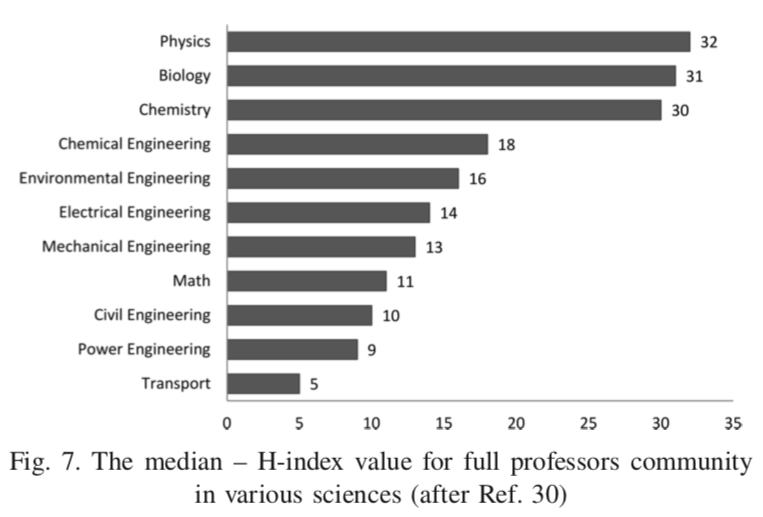
\includegraphics[scale=0.35]{figs/03/median-h}
\caption{Fonte: (Czarnecki, 2013) et al.}
\end{figure}

\end{frame}

%%
\begin{frame}{Altimetrias}
Altimetrias (\textit{altmetrics}) são métricas alternativa que fogem ao padrão e buscam outras variáveis.

Ver \url{https://doi.org/10.18617/liinc.v9i1.569}
\end{frame}

%%
\section{CAPES Qualis}

\begin{frame}{Ranking de periódicos}
\begin{block}{O que é?}
Sistema usado para classificar a produção científica dos programas de pós-graduação no que se refere aos artigos publicados em periódicos científicos.
\end{block}
\begin{block}{Para que serve?}
Avaliar a produção científica dos programas de pós-graduação a partir da análise de qualidade dos periódicos.
\end{block}
\begin{block}{Estratos atuais}
A1, A2; B1, B2, B3, B4, B5, C
\end{block}

Ver: \url{http://qualis.capes.gov.br}
\end{frame}


\subsection{Novas regras de avaliação}

%%
\begin{frame}{Proposta de aprimoramento}
\begin{itemize}
\item Necessidade de novo modelo de avaliação da pós-graduação (out/2018) - PNPG 2011 - 2020
\end{itemize}
\begin{quotation}
``(...) apesar dos excelentes resultados obtidos até o presente, o \textbf{atual sistema avaliativo atingiu um esgotamento e deve ser conceitual e objetivamente repensado e aprimorado}.''
\end{quotation}

\scriptsize{\url{https://www.capes.gov.br/36-noticias/9370-mudancas-na-ficha-de-avaliacao-valorizam-qualidade-dos-programas}}
\end{frame}

%%
\begin{frame}{Novo documento (dez/2018)}
\begin{itemize}
\item PPGs serão avaliados mediante 3 quesitos
\begin{enumerate}
\item \textbf{Programa:} funcionamento, estrutura e planejamento estratégico;
\item \textbf{Formação:} qualidade de teses, dissertações e produção de discentes, docentes e egressos;
\item \textbf{Impacto na sociedade:} caráter inovador da produção, efeitos econômicos, internacionalização e visibilidade;
\end{enumerate}
\end{itemize}
\end{frame}

%%
\begin{frame}{Avaliação multidimensional}
Até 2021, teremos uma fase de transição para a \textbf{Avaliação Multidimensional} visando a
Avaliação Quadrienal 2021 - 2024:
\begin{figure}
\centering
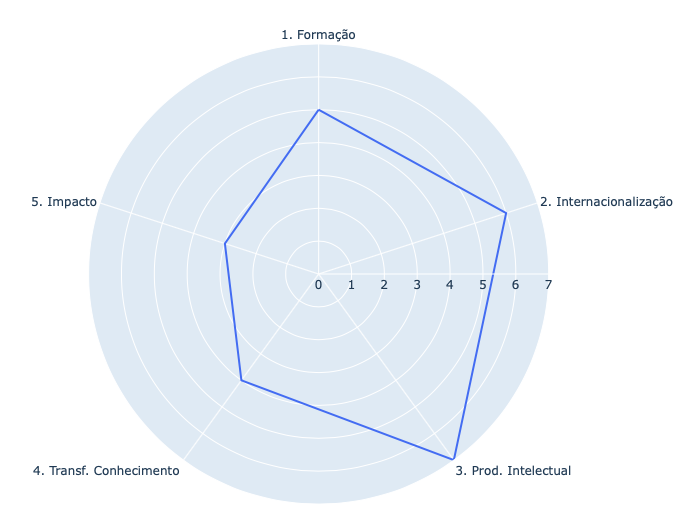
\includegraphics[scale=0.3]{figs/03/multidimensional}
\end{figure}
\end{frame}

%%
\begin{frame}{Área: Engenharias III}
Área composta por:

\begin{itemize}
\item Engenharia Mecânica
\item Engenharia de Produção
\item Engenharia Naval e Oceânica
\item Engenharia Aeroespacial
\end{itemize}
\end{frame}

\subsection{O novo Qualis}

%%
\begin{frame}{Qualis até 2016}
\begin{itemize}
\item Classificações distintas para um mesmo periódico entre as áreas
\item Diversidade de critérios utilizados para classificação
\item Falta de comparabilidade entre áreas
\end{itemize}
\end{frame}

%%
\begin{frame}{O novo Qualis}
\begin{itemize}
\item \textbf{Estratificação única} para cada periódico
\item Baseado em \textbf{indicadores universais}
\item Estrato é função dos \textbf{percentis nas bases JCR e Scopus}
\item Metodologia:
\begin{itemize}
\item Maior percentil entre bases JCR e Scopus
\item Em cada base: maior percentis entre áreas em que se enquadra
\end{itemize}
\end{itemize}
\end{frame}

%%
\begin{frame}{Nova estratificação}
\begin{figure}
\centering
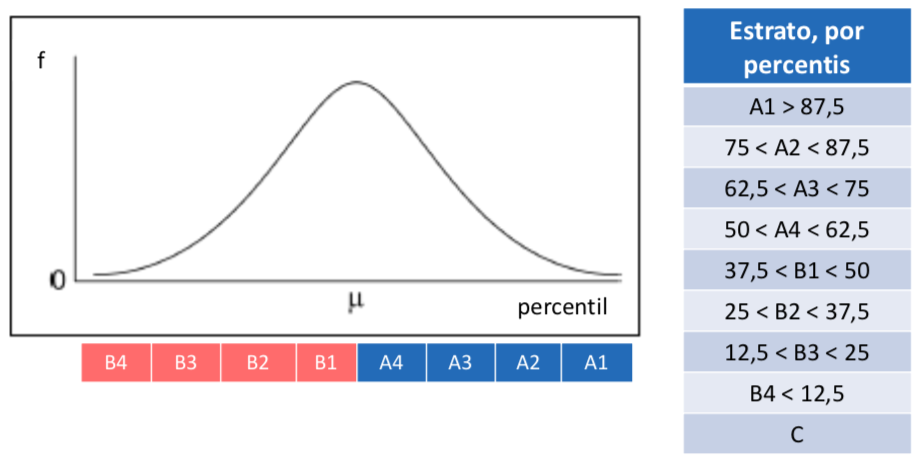
\includegraphics[scale=0.35]{figs/03/estratos}
\end{figure}
\end{frame}

\subsection*{O índice H2}

%%
\begin{frame}{Perfil do corpo docente}
\begin{figure}
\centering
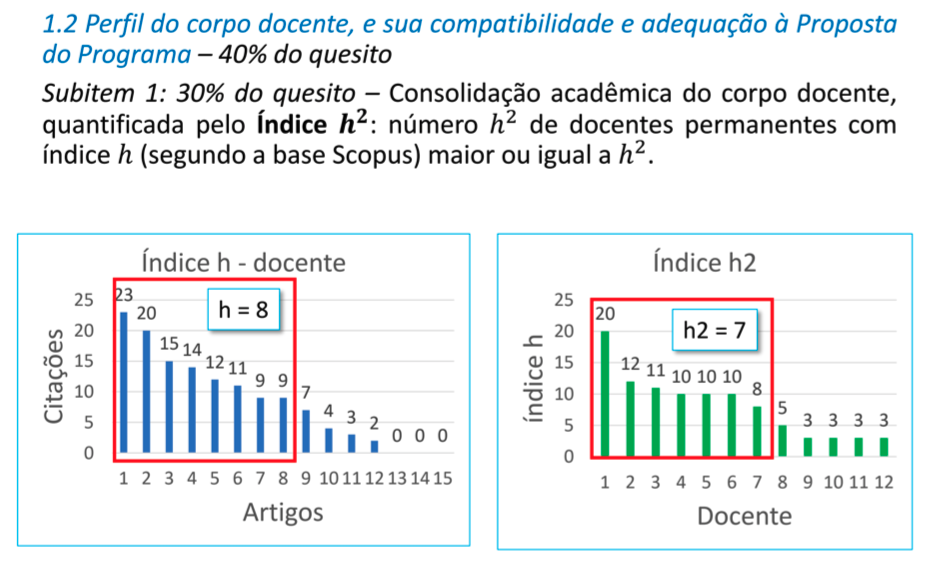
\includegraphics[scale=0.35]{figs/03/indice-h2}
\end{figure}
\end{frame}

\subsection*{Papel do pós-graduando no PPGEM/UFPB}

%%
\begin{frame}{Avaliação de sua formação}
\begin{itemize}
\item Qualidade e adequação das teses, dissertações ou equivalente em relação às áreas de concentração e linhas de pesquisa do programa
\begin{itemize}
\item Questionário da Banca Examinadora
\item Nível dos membros da BE
\item Prêmios, distinções e reconhecimentos acadêmicos
\end{itemize}
\end{itemize}
\end{frame}

%%
\begin{frame}
\begin{itemize}
\item Qualidade da produção intelectual de discentes e egressos
\begin{itemize}
\item Indicação das melhores teses e dissertações
\item Artigos com melhor qualificação
\item Trabalhos em eventos nacionais/internacionais
\item Publicações indexadas na Scopus ou WoS
\end{itemize}
\end{itemize}
\end{frame}

%%
\begin{frame}
\begin{itemize}
\item Destino, atuação e avaliação dos egressos do programa em relação à formação recebida
\begin{itemize}
\item Casos de sucesso de egressos
\item Titulações
\end{itemize}
\end{itemize}
\end{frame}

%%
\begin{frame}
\begin{itemize}
\item Qualidade das atividades de pesquisa e da produção intelectual do corpo docente no programa
\begin{itemize}
\item Capacidade de captação de recursos e valores de financiamento
\item Contribuições diretamente aplicáveis e produtos (produção técnica)
\item Patentes, softwares, material didático, relatório, etc.
\end{itemize}
\end{itemize}
\end{frame}


%%
\begin{frame}
\begin{itemize}
\item Qualidade e envolvimento do corpo docente em relação às atividades
de formação no programa
\begin{itemize}
\item Avaliações qualitativas sobre relação docente/discente
\item Eventos, seminários, avaliações
\end{itemize}
\end{itemize}
\end{frame}

%%
\begin{frame}{Impacto do PPG}
\begin{figure}
\centering
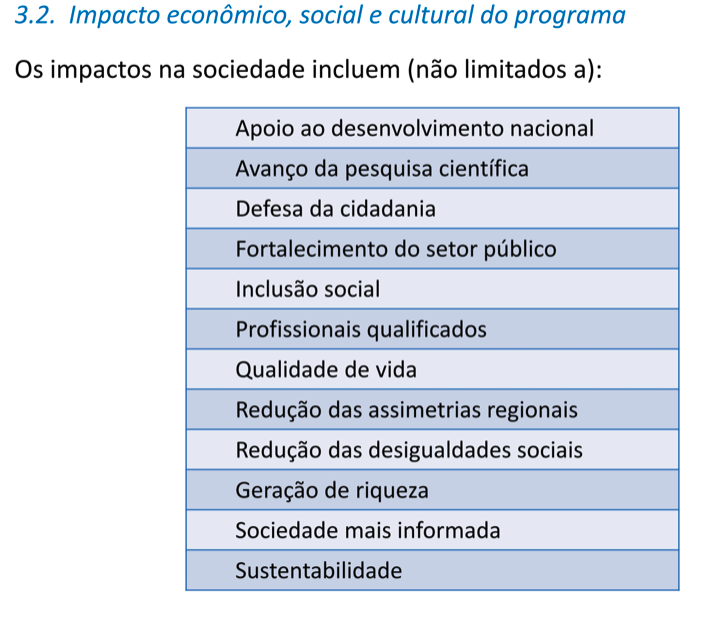
\includegraphics[scale=0.35]{figs/03/impactos}
\end{figure}
\end{frame}


\section{CAPES Periódicos: Hands-on}

\subsection{Base WoS}

%%
\begin{frame}{Praticando na base WoS}
\begin{enumerate}
\item Acessar portal \url{capes.periodicos.gov.br}
\item Fazer login via CAFe
\item Buscar base \textit{Web of Science}
\item Realizar pesquisas
\item Verificar percentis
\end{enumerate}
\end{frame}

\subsection{Base Scopus}

%%
\begin{frame}{Praticando na base Scopus}
\begin{enumerate}
\item Acessar portal \url{capes.periodicos.gov.br}
\item Fazer login via CAFe
\item Buscar base \textit{Scopus}
\item Realizar pesquisas
\item Verificar percentis
\end{enumerate}
\end{frame}


\begin{frame}{Desafio}

A turma se anima a fazer um arquivo como este para a Engenharia no Brasil? 

\url{https://www.degruyter.com/downloadpdf/j/bpasts.2013.61.issue-1/bpasts-2013-0001/bpasts-2013-0001.pdf}

\end{frame}

%%
\begin{frame}{Leitura recomendada}

\url{http://www.leidenmanifesto.org}

\end{frame}

%% === REFS
\begin{frame}[allowframebreaks]
\frametitle{Referências}
\begin{thebibliography}{9}
\setbeamertemplate{bibliography item}[book]
%
\bibitem{falbo2018}Hood, W., Wilson, C. \textit{The literature of bibliometrics, scientometrics, and informetrics}. Scientometrics, 52:2, 2001.
\bibitem{vanti2002}Vanti, N. A. P. \textit{Da bibliometria à webometria: uma exploração conceitual dos mecanismos utilizados para medir o registro da informação e a difusão do conhecimento}, Ci. Inf., Brasília, 31(2), p. 152-162, mai/ago, 2002.
\end{thebibliography}
\end{frame}